\documentclass[aspectratio=169,11pt,t]{beamer}
% ============================================================
%  ksa-cs-v2: ksa-cs-lecture-template.tex 스타일 + 한글, v2 덱(16:9)용.
%    - 짙은 네이비 헤드라인 (섹션 이름 + 프레임마다 점)
%    - 꽉 찬 파란 제목 막대, 둥근 그림자 블록
%    - 한글: Noto Sans CJK KR (fontspec)
%  사용:
%    \documentclass[aspectratio=169,11pt,t]{beamer}
%    \input{<..>/theme/ksa-cs-v2.tex}
%  ksa-theme.tex 의 매크로(\kb \kq, ksablue/ksared 등)도 같은 이름으로 둔다
%  -> v2 덱 본문을 거의 그대로 옮길 수 있다.
% ============================================================

\usepackage{fontspec}
\usepackage{amsmath,amssymb}
\usepackage{tikz}
\usepackage{listings}
\usepackage{graphicx}
\usepackage{booktabs}
\usepackage{varwidth}
% enumitem 은 넣지 않는다 (beamer 글머리표가 사라진다)

\defaultfontfeatures{Ligatures=TeX}
\setmainfont{Noto Sans CJK KR}
\setsansfont{Noto Sans CJK KR}
\setmonofont{Noto Sans Mono CJK KR}[Scale=0.92]
\usefonttheme{professionalfonts}

% ---------- 기본 틀 ----------
\usetheme{default}
\useinnertheme[shadow=true]{rounded}
\setbeamertemplate{navigation symbols}{}
\setbeamersize{text margin left=1em,text margin right=1em}

% ---------- 색 (템플릿 원본 값) ----------
\definecolor{navydark}{HTML}{191959}
\definecolor{navydim}{HTML}{8888B0}
\definecolor{navytitle}{HTML}{262686}
\definecolor{navyblue}{HTML}{3333B2}
\definecolor{blockbodybg}{HTML}{E9E9F3}
\definecolor{examplegreen}{HTML}{006000}
\definecolor{examplebg}{HTML}{E5EFE5}
\definecolor{alertred}{HTML}{BF0000}
\definecolor{alertbg}{HTML}{F9E5E5}
% ksa-theme.tex 와 같은 이름 (본문 호환)
\colorlet{ksablue}{navytitle}
\colorlet{ksabluedk}{navydark}
\definecolor{ksagold}{HTML}{D6CBB1}
\definecolor{ksagolddk}{HTML}{A9976B}
\colorlet{ksared}{alertred}
\definecolor{ksagray}{HTML}{5B5B5B}

\setbeamercolor{structure}{fg=navyblue}
\setbeamercolor{alerted text}{fg=alertred}
\setbeamercolor{frametitle}{bg=navytitle,fg=white}
\setbeamercolor{title}{fg=white,bg=navytitle}
\setbeamercolor{block title}{bg=navytitle,fg=white}
\setbeamercolor{block body}{bg=blockbodybg,fg=black}
\setbeamercolor{block title example}{bg=examplegreen,fg=white}
\setbeamercolor{block body example}{bg=examplebg,fg=black}
\setbeamercolor{block title alerted}{bg=alertred,fg=white}
\setbeamercolor{block body alerted}{bg=alertbg,fg=black}
\setbeamercolor{item}{fg=navyblue}
\setbeamertemplate{itemize item}[circle]
\setbeamertemplate{itemize subitem}[triangle]

% ---------- 헤드라인: miniframes (섹션 이름 + 점) ----------
\useoutertheme[subsection=false]{miniframes}
\setbeamerfont{section in head/foot}{size=\tiny}
\setbeamercolor{section in head/foot}{bg=navydark,fg=white}
\setbeamercolor{mini frame}{fg=white}
\setbeamertemplate{mini frames}[circle]

% ---------- 제목 막대: 폭 꽉 채움, 두 줄까지 ----------
\setbeamerfont{frametitle}{size=\normalsize,series=\bfseries}
\setbeamertemplate{frametitle}{%
  \nointerlineskip
  \begin{beamercolorbox}[wd=\paperwidth,ht=2.7ex,dp=1.1ex,leftskip=.3cm,rightskip=.3cm]{frametitle}%
    \usebeamerfont{frametitle}\insertframetitle
  \end{beamercolorbox}}

% ---------- 쪽 번호: 오른쪽 아래 ----------
\setbeamertemplate{footline}{%
  \hfill
  {\color{navydim}\scriptsize\insertframenumber\,/\,\inserttotalframenumber}%
  \hspace{3mm}\vspace{2mm}%
}

% ---------- 표지: 템플릿처럼 헤드라인은 그대로, 가운데 둥근 그림자 상자에 제목 한 줄 ----------
% 덱에서:  {\setbeamertemplate{footline}{}\begin{frame}[c,noframenumbering]\titlepage\end{frame}}
\setbeamercolor{title}{fg=white,bg=navyblue}
\makeatletter
\setbeamertemplate{title page}{%
  \vfill
  \centering
  \begin{minipage}{0.84\paperwidth}
  \begin{beamercolorbox}[wd=\linewidth,sep=7pt,center,rounded=true,shadow=true]{title}
    {\usebeamerfont{title}\inserttitle\par}%
    \ifx\insertsubtitle\@empty\else\vskip0.4em{\usebeamerfont{subtitle}\insertsubtitle\par}\fi
  \end{beamercolorbox}
  \end{minipage}\par\vskip1.6em
  {\usebeamerfont{author}\color{navytitle}\insertauthor\par}\vskip0.3em
  {\usebeamerfont{institute}\color{ksagray}\insertinstitute\par}
  \vfill
}
\makeatother
\setbeamerfont{title}{series=\bfseries,size=\Large}
\setbeamerfont{subtitle}{size=\normalsize}
\setbeamerfont{author}{size=\normalsize}
\setbeamerfont{institute}{size=\small}

% ksa-theme 호환: 덱이 \renewcommand{\ksacredit}{..} 를 해도 되게 (꼬리말에는 안 쓴다)
\newcommand{\ksacredit}{}

% ---------- 강조 ----------
\newcommand{\hl}[1]{\textcolor{alertred}{#1}}
\newcommand{\hlb}[1]{\textcolor{navyblue}{#1}}
\newcommand{\kb}[1]{\textbf{\color{ksablue}#1}}
\newcommand{\kq}[1]{\textbf{\color{ksared}#1}}

% ---------- 파이썬 코드 (템플릿과 같은 색) ----------
\definecolor{codekw}{HTML}{0033B3}
\definecolor{codebuiltin}{HTML}{BF0000}
\definecolor{codestr}{HTML}{067D17}
\definecolor{codecomment}{HTML}{8C8C8C}
\definecolor{codenum}{HTML}{1750EB}
\lstdefinestyle{py}{
  language=Python, basicstyle=\ttfamily\scriptsize,
  keywordstyle=\color{codekw}\bfseries, stringstyle=\color{codestr},
  commentstyle=\color{codecomment}\itshape, numberstyle=\color{codenum},
  emph={print,len,range,sum,input,int,str,float,list,dict,append,remove,sorted,abs,min,max},
  emphstyle=\color{codebuiltin}, showstringspaces=false, keepspaces=true,
  columns=fixed, basewidth=0.52em, aboveskip=1mm, belowskip=1mm, xleftmargin=2mm,
  breaklines=true
}
\lstset{style=py}

% 원본 덱 (ksa-theme): slides/v2/ml1/week02/overfitting/ -- 그림은 거기 figs/ 를 그대로 쓴다
\setbeamerfont{author}{size=\normalsize}
\setbeamerfont{institute}{size=\small}
\graphicspath{{../../../v2/ml1/week02/overfitting/figs/}{../../../assets/}}
\makeatletter
\newcommand{\markpage}[1]{\protected@write\@auxout{}{\string\newlabel{#1}{{\the\c@framenumber}{}}}\hypertarget{#1}{}}
\newcommand{\pref}[1]{\hyperlink{#1}{\textcolor{ksagolddk}{(p.\ref{#1})}}}
\makeatother

\renewcommand{\ksacredit}{Machine Learning and Deep Learning \,\textperiodcentered\, 과대적합과 과소적합}
\title{과대적합과 과소적합 (Overfitting \& Underfitting)}
\subtitle{완벽한 곡선이 새 데이터를 틀리는 이유, 그리고 교차 검증}
\author{Machine Learning and Deep Learning}
\institute{한국과학영재학교 (KSA)}
\date{}
\begin{document}
{\setbeamertemplate{footline}{}\begin{frame}[c,noframenumbering]\titlepage\end{frame}}

\section{질문}
% --- 오늘의 질문
\begin{frame}{오늘의 질문}
\vfill
\centering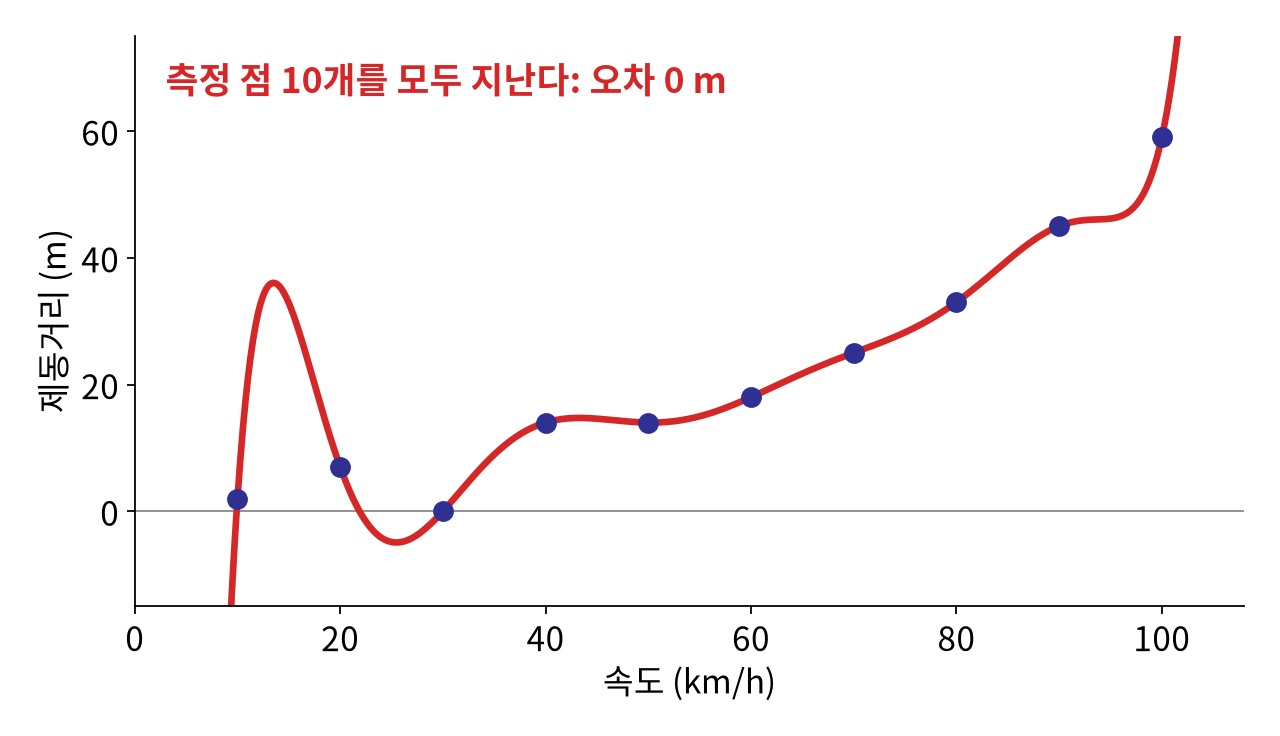
\includegraphics[width=0.62\linewidth]{of_hook.png}\par\vskip0.3em
{\large 측정한 점을 모두 지나는 곡선. \kq{이 모델로 처음 보는 속도의 제동거리도 맞힐 수 있을까?}}
\vfill
\note{자동차 속도에 따른 제동거리를 10번 재서 점으로 찍었습니다. 빨간 곡선은 이 점 10개를 하나도 빠짐없이 지나갑니다. 측정 데이터에서는 오차가 0미터, 완벽합니다. 그런데 이 모델로 처음 보는 속도의 제동거리를 맞힐 수 있을까요? 오늘은 이 질문에서 시작해서 과대적합, 과소적합, 그리고 둘 사이에서 모델을 고르는 교차 검증까지 갑니다.}
\end{frame}

\section{세 모델}
% --- 데이터
\begin{frame}{제동거리: 속도가 2배면 4배}
\markpage{data}
\vfill
\centering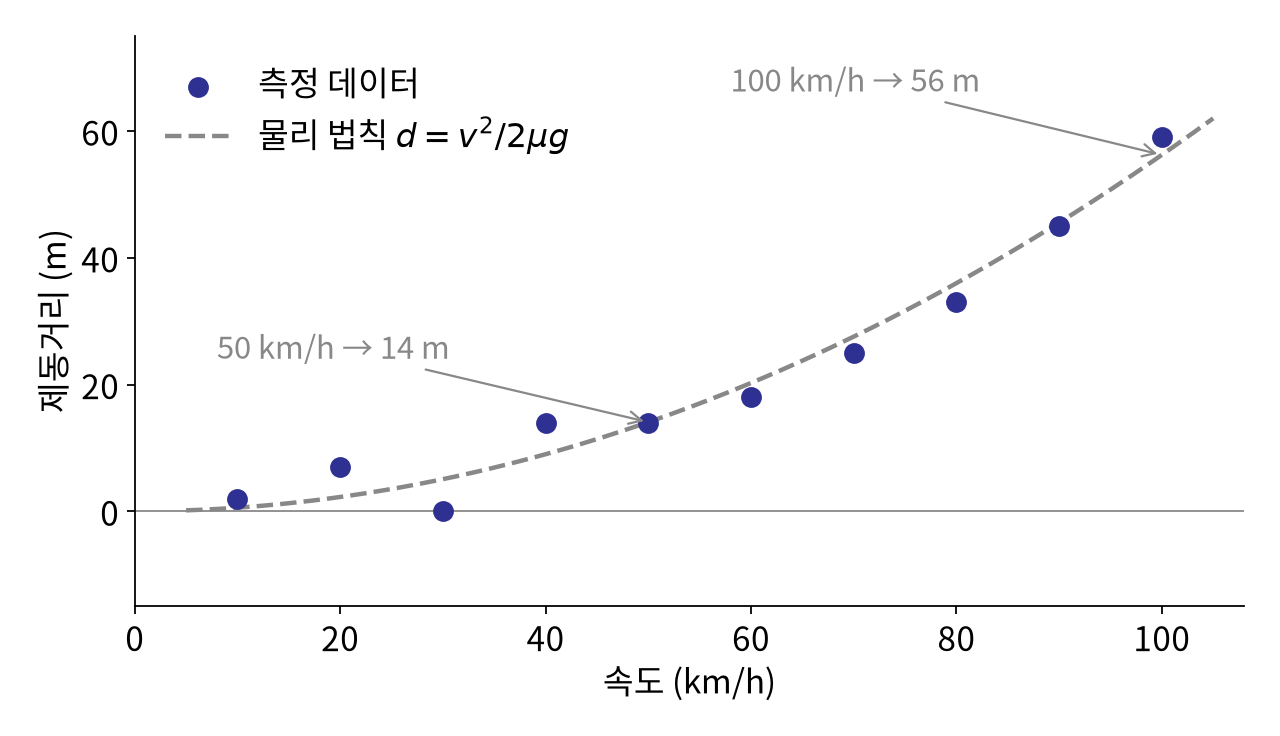
\includegraphics[width=0.58\linewidth]{of_data.png}\par\vskip0.2em
{\large 제동거리 = 브레이크를 밟고 멈출 때까지 가는 거리 \qquad $d = \dfrac{v^2}{2\mu g}$}\\[0.3em]
{\small $v$: 속도 \quad $\mu = 0.7$: 마른 아스팔트의 마찰계수 (가정) \quad $g$: 중력가속도 \quad 점: 법칙 + 측정 오차 (예시)}
\vfill
\note{제동거리는 브레이크를 밟고 완전히 멈출 때까지 가는 거리입니다. 물리 법칙으로는 속도의 제곱에 비례합니다. 그래서 50킬로에서 14미터면 100킬로에서는 4배인 56미터입니다. 회색 점선이 이 법칙이고, 파란 점은 법칙에 측정 오차를 더한 예시 데이터입니다. 30킬로에서 0미터처럼 이상한 점도 있는데, 실제 측정에서도 이런 잡음은 늘 섞입니다. 오늘은 이 진짜 규칙을 모른다고 치고 점 10개만 보고 모델을 고릅니다.}
\end{frame}

% --- 직선
\begin{frame}{직선으로 맞추면: 과소적합}
\vfill
\centering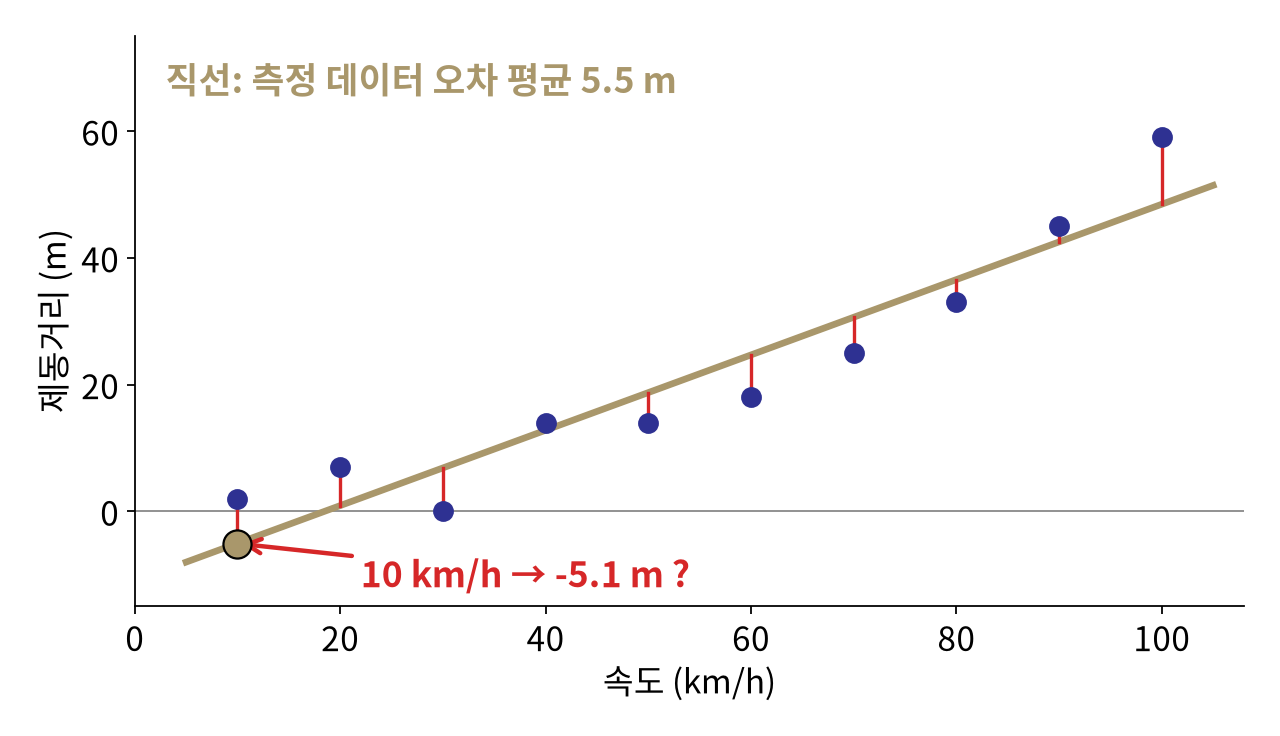
\includegraphics[width=0.6\linewidth]{of_line.png}\par\vskip0.3em
{\large 10 km/h 에서 실제 2 m 를 \kq{$-5.1$ m} 로 예측 \quad $\to$ 제동거리가 음수? \quad \kb{너무 단순하다}}
\vfill
\note{먼저 1주차에 배운 직선을 그어 봅니다. 가운데는 그럭저럭 맞는데, 10킬로에서 실제 2미터를 마이너스 5.1미터로 예측합니다. 제동거리가 음수일 수는 없으니 명확히 틀린 예측입니다. 빨간 선이 각 점의 오차인데, 양 끝에서는 직선이 점 아래, 가운데서는 점 위에 있습니다. 데이터가 휘어 있는데 직선은 휠 수가 없어서입니다. 이렇게 모델이 너무 단순해서 가진 데이터조차 못 따라가는 것을 과소적합, underfitting이라고 합니다.}
\end{frame}

% --- 오차
\begin{frame}{오차를 숫자 하나로: 평균 절대 오차}
\markpage{mae}
\vfill
\centering
{\LARGE\[ \text{MAE} = \frac{1}{m}\sum_{i=1}^{m}\big|\,h(x^{(i)}) - y^{(i)}\,\big| \]}\vskip0.6em
{\large 10 km/h: \; $|\,{-5.1} - 2\,| = 7.1$ m \qquad 점 10개의 평균 \; $\to$ \kb{5.5 m}}\\[0.8em]
{\small $m$: 데이터 수 \quad 절댓값: 위로 틀리든 아래로 틀리든 같은 거리 \quad 단위가 미터 그대로라 읽기 쉽다}
\vfill
\note{오차를 숫자 하나로 말하기 위해 평균 절대 오차, MAE를 씁니다. 각 점에서 예측과 실제의 차이에 절댓값을 씌우고 평균을 냅니다. 10킬로에서는 마이너스 5.1과 2의 차이, 7.1미터입니다. 점 10개 모두 이렇게 재서 평균을 내면 직선은 5.5미터입니다. 선형회귀 시간의 RMSE와 비슷하지만 제곱 대신 절댓값이라서, 큰 오차 하나에 덜 휘둘리고 단위가 미터 그대로라 읽기 쉽습니다. 오늘은 이 숫자로 모델을 비교합니다.}
\end{frame}

% --- 새 데이터
\begin{frame}{구불구불 곡선을 새 데이터에 대 보면}
\vfill
\centering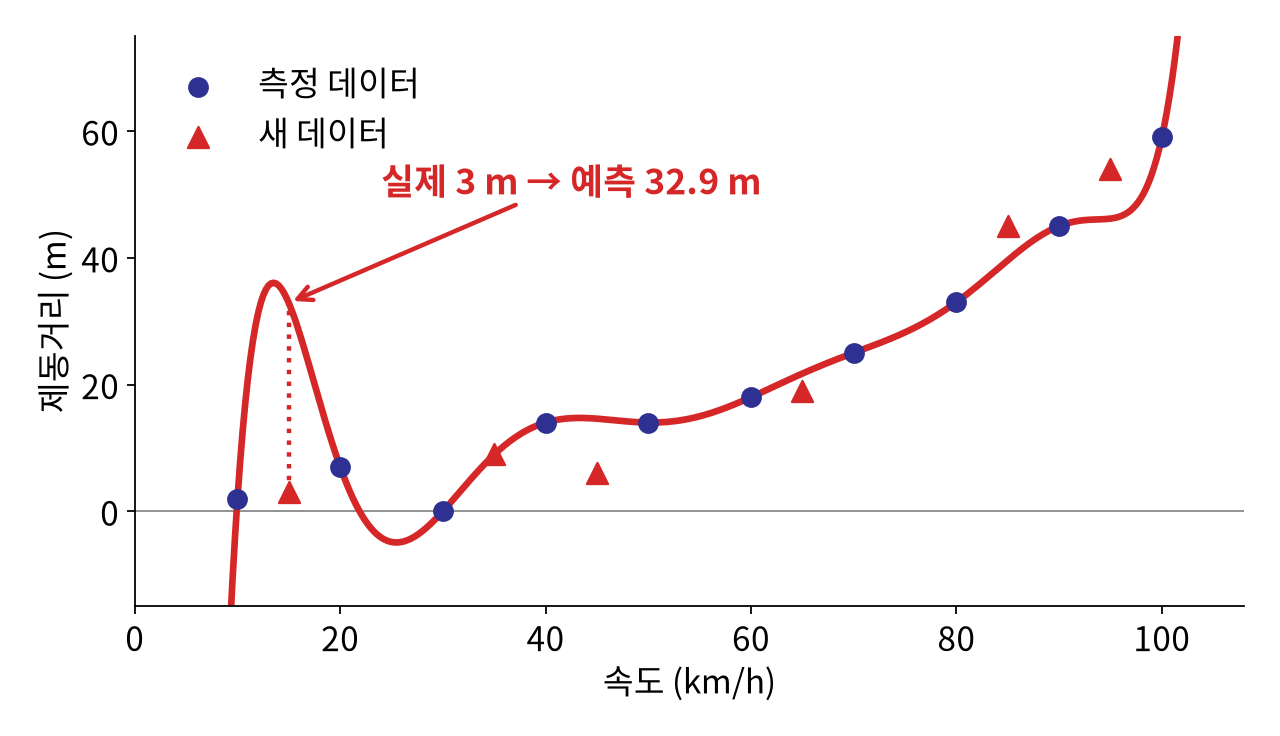
\includegraphics[width=0.6\linewidth]{of_new.png}\par\vskip0.3em
{\large 측정 데이터 오차 \kb{0 m} \quad 새 데이터 6개 오차 \kq{9.1 m} \qquad 15 km/h 에서 3 m 를 32.9 m 로}
\vfill
\note{이번에는 처음의 구불구불한 곡선입니다. 9차 다항식이라 측정 점 10개를 모두 지나고 오차는 0미터입니다. 그런데 새로 잰 데이터 6개, 빨간 삼각형을 대 보면 이야기가 달라집니다. 15킬로에서 실제 3미터인데 곡선은 약 33미터를 예측합니다. 점과 점 사이에서 곡선이 크게 출렁이기 때문입니다. 새 데이터의 평균 오차는 9.1미터로, 직선보다도 나쁩니다. 측정한 점을 외워 버린 겁니다. 이걸 과대적합, overfitting이라고 합니다.}
\end{frame}

% --- 2차
\begin{frame}{2차 곡선: 물리 법칙과 같은 모양}
\vfill
\centering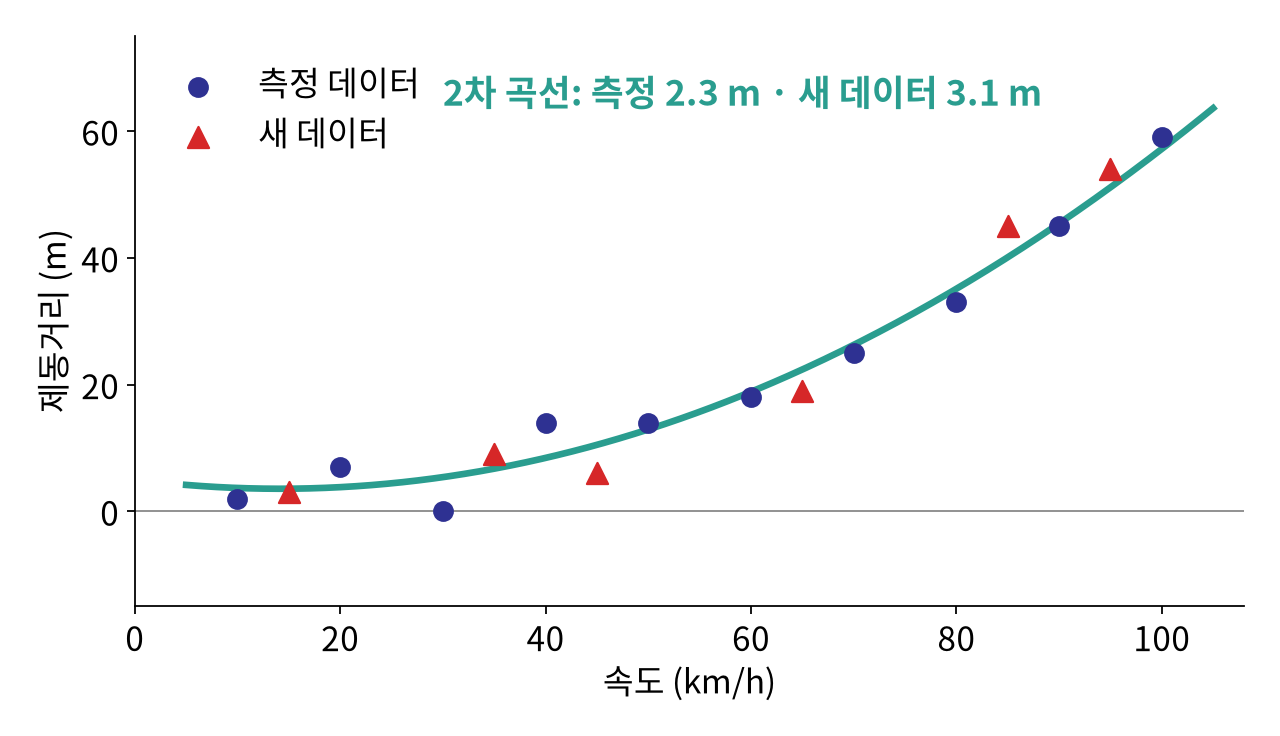
\includegraphics[width=0.6\linewidth]{of_quad.png}\par\vskip0.3em
{\large $h(x) = w_0 + w_1 x + w_2 x^2$ \qquad 측정 \kb{2.3 m} \quad 새 데이터 \kb{3.1 m}}
\vfill
\note{2차 곡선은 어떨까요. 측정 데이터에서는 2.3미터로 구불구불 곡선보다 오차가 큽니다. 모든 점을 지나지는 않으니까요. 그런데 새 데이터에서는 3.1미터로 셋 중 가장 작습니다. 속도의 제곱이라는 물리 법칙과 같은 모양이라서, 점을 외우지 않고 규칙을 배운 겁니다.}
\end{frame}

% --- 표
\begin{frame}{세 모델의 성적표}
\markpage{table}
\vfill
\centering
{\Large\begin{tabular}{lccc}
 & 직선 & 2차 곡선 & 구불구불 곡선 (9차)\\\hline\\[-0.8em]
측정 데이터 오차 & 5.5 m & 2.3 m & \kb{0 m}\\[0.4em]
새 데이터 오차 & 6.4 m & \kb{3.1 m} & \kq{9.1 m}
\end{tabular}}\vskip1.2em
{\large 측정 데이터에서 1등 $\neq$ 새 데이터에서 1등}
\vfill
\note{세 모델을 표로 모았습니다. 측정 데이터 오차만 보면 구불구불 곡선이 0미터로 1등입니다. 하지만 우리가 정말 원하는 건 처음 보는 데이터를 맞히는 것이고, 새 데이터에서는 2차 곡선이 3.1미터로 1등, 구불구불 곡선은 9.1미터로 꼴찌입니다. 학습에 쓴 데이터의 오차는 모델이 얼마나 좋은지 알려 주지 못합니다.}
\end{frame}

% --- 세 모델 나란히
\begin{frame}{너무 단순하거나, 너무 외우거나}
\vfill
\centering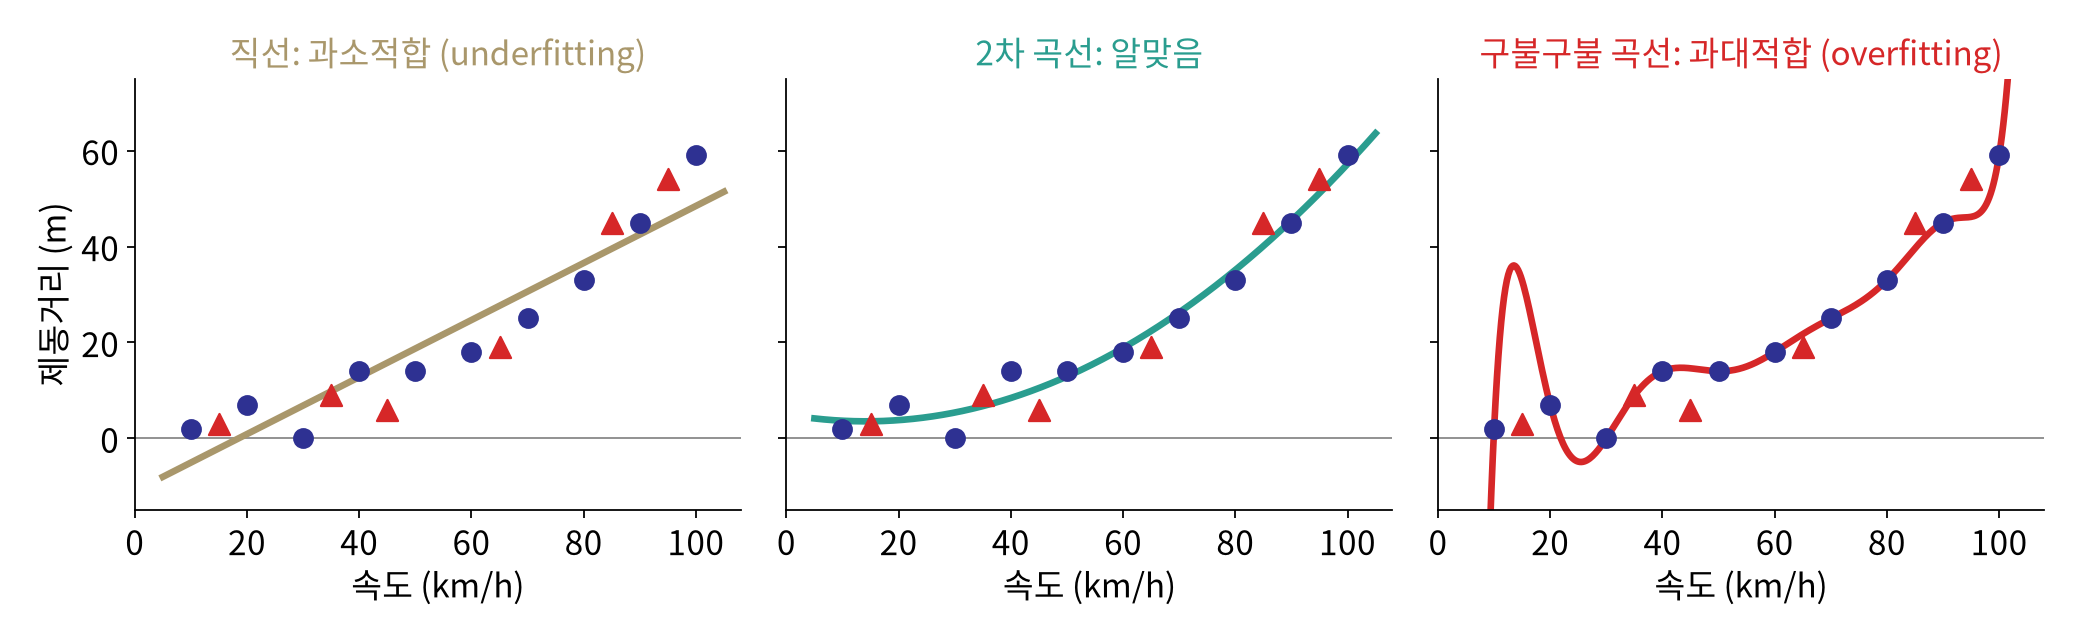
\includegraphics[width=0.95\linewidth]{of_three.png}\par\vskip0.3em
{\large \kb{과소적합}: 가진 데이터도 못 따라간다 \qquad \kq{과대적합}: 가진 데이터를 외워서 새 데이터를 틀린다}
\vfill
\note{세 모델을 나란히 놓았습니다. 왼쪽 직선은 너무 단순해서 측정 데이터조차 못 따라가는 과소적합입니다. 오른쪽 9차 곡선은 측정 데이터를 외워서 새 데이터를 틀리는 과대적합입니다. 가운데 2차 곡선이 둘 사이의 알맞은 복잡도입니다. 과소적합은 측정 오차와 새 데이터 오차가 둘 다 크고, 과대적합은 측정 오차는 작은데 새 데이터 오차만 큽니다. 이 차이로 둘을 구별합니다.}
\end{frame}

% --- 왜 외울 수 있나
\begin{frame}{9차 곡선은 왜 점을 외울 수 있나}
\vfill
\centering
{\Large\[ h(x) = \underbrace{w_0 + w_1 x + w_2 x^2 + \cdots + w_9 x^9}_{\text{10 weights}} \]}\vskip0.6em
{\large 숫자 10개를 마음대로 고를 수 있다 \quad = \quad 점 10개를 \kq{정확히} 지나게 할 수 있다}\\[0.8em]
{\normalsize 직접 만들기: 점 $x_1$ 에서만 $y_1$, 나머지 9개 점에서는 0 \;$\to$\; $y_1\,\dfrac{(x-x_2)(x-x_3)\cdots(x-x_{10})}{(x_1-x_2)(x_1-x_3)\cdots(x_1-x_{10})}$}\\[0.3em]
{\normalsize 괄호가 \kb{9개} $\to$ 9차. \quad 점 10개 몫을 이렇게 하나씩 만들어 더하면 끝}\\[0.8em]
{\small 잡음까지 그대로 따라가느라 점 사이에서 출렁인다 \qquad 데이터가 많아지면 외우기 어려워진다}
\vfill
\note{9차 곡선이 점을 외울 수 있는 이유는 간단합니다. 9차 다항식에는 w0부터 w9까지 숫자가 10개 있습니다. 점이 10개면 방정식 10개, 미지수 10개라서 모든 점을 정확히 지나는 곡선을 항상 찾을 수 있습니다. 직접 만들 수도 있습니다. 첫 번째 점에서만 y1이고 나머지 9개 점에서는 0이 되는 식은, 나머지 점들로 x 빼기 x2부터 x 빼기 x10까지 곱하면 됩니다. 괄호가 9개라서 9차입니다. 점 10개를 모두 곱하면 10차가 되지만, 그러면 모든 점에서 0이 되어 버려서 점을 지나는 곡선이 아닙니다. 점마다 이런 조각을 하나씩 만들어 더하면 10개 점을 모두 지나는 9차 곡선이 됩니다. 문제는 측정 오차, 즉 잡음까지 그대로 따라간다는 겁니다. 30킬로에서 0미터 같은 잡음을 지나려고 곡선이 휘고, 그래서 점 사이에서 출렁입니다. 반대로 데이터가 1000개라면 숫자 10개로 다 외울 수는 없습니다. 그래서 과대적합은 데이터에 비해 모델이 복잡할 때 생깁니다.}
\end{frame}

\section{교차 검증}
% --- 새 데이터는 없다
\begin{frame}{문제: 새 데이터는 미리 없다}
\vfill
\centering
{\Large 모델을 고를 때는 아직 \kq{새 데이터}가 없다}\\[1.0em]
{\large 그러면 \kb{가진 데이터 일부를 숨겨 두고}, 숨긴 데이터로 시험한다}\\[1.0em]
{\small 숨긴 데이터 = 검증 데이터 (validation) \qquad 학습에는 절대 쓰지 않는다}
\vfill
\note{지금까지는 새로 잰 데이터가 있어서 비교할 수 있었습니다. 그런데 실제로 모델을 고를 때는 아직 새 데이터가 없습니다. 미래의 데이터니까요. 그러면 어떻게 할까요? 가진 데이터 중 일부를 숨겨 두고, 나머지로 학습한 다음, 숨긴 데이터로 시험합니다. 숨긴 데이터를 검증 데이터라고 부릅니다. 핵심은 검증 데이터를 학습에 절대 쓰지 않는 겁니다. 그래야 새 데이터를 흉내 낼 수 있습니다.}
\end{frame}

% --- 5겹 교차 검증
\begin{frame}{5겹 교차 검증: 돌아가며 한 조각씩 숨기기}
\markpage{cv}
\vfill
\centering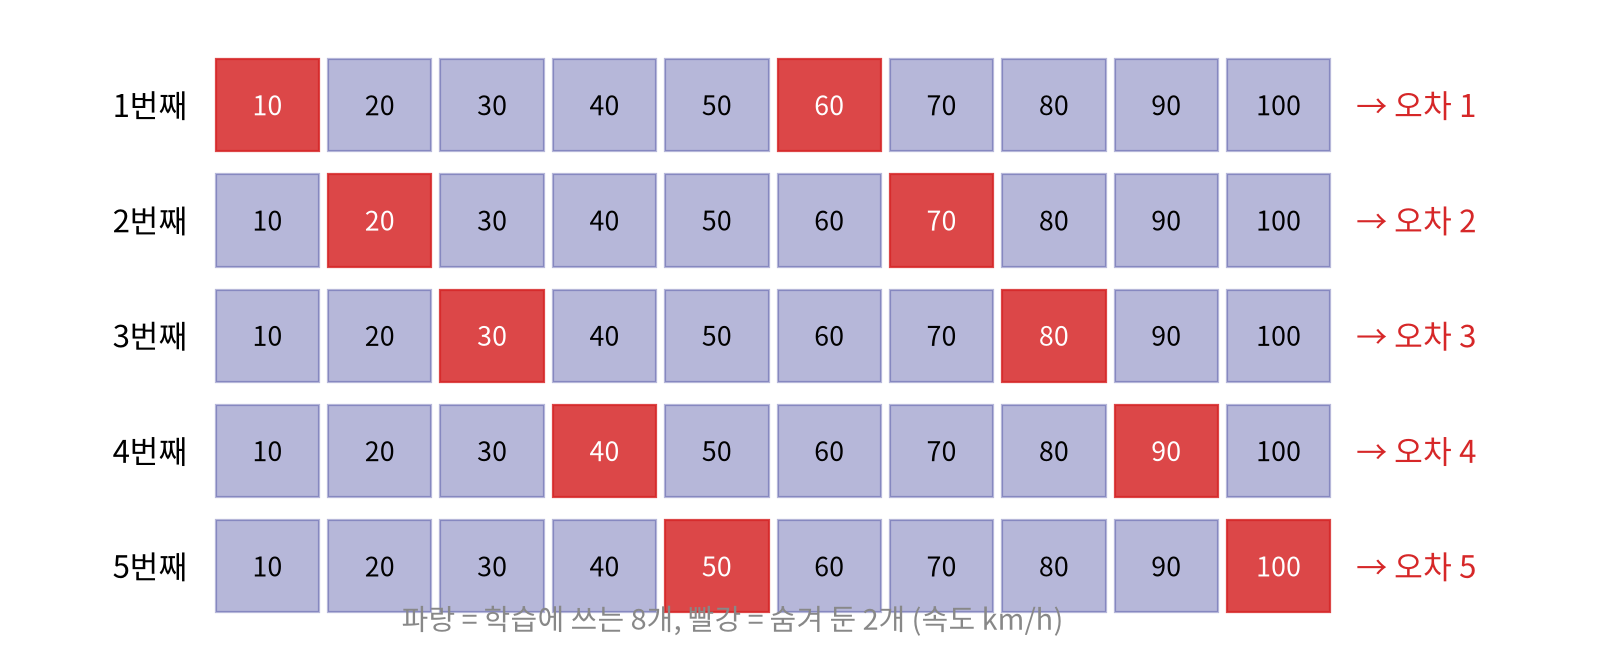
\includegraphics[width=0.56\linewidth]{of_folds.png}\par\vskip0.1em
{\large\[ \text{CV} = \frac{1}{5}\sum_{k=1}^{5} \text{MAE}_k \]}
{\small 점 10개 $\to$ 2개씩 5조각. 한 조각은 숨기고 8개로 학습 $\to$ 숨긴 2개의 오차. 다섯 번 반복해서 평균 (k-fold cross validation)}
\vfill
\note{점이 10개뿐이라 한 번만 숨기면 운에 따라 결과가 크게 달라집니다. 그래서 돌아가며 숨깁니다. 점 10개를 2개씩 5조각으로 나누고, 첫 번째에는 10킬로와 60킬로를 숨기고 나머지 8개로 학습해서 숨긴 2개의 오차를 잽니다. 두 번째에는 20과 70을 숨기고, 이렇게 다섯 번 하면 모든 점이 한 번씩 검증 데이터가 됩니다. 다섯 오차의 평균이 교차 검증 오차입니다. 5조각이라서 5겹 교차 검증, k-fold cross validation이라고 부릅니다.}
\end{frame}

% --- 교차 검증 결과
\begin{frame}{교차 검증으로 고르기}
\vfill
\centering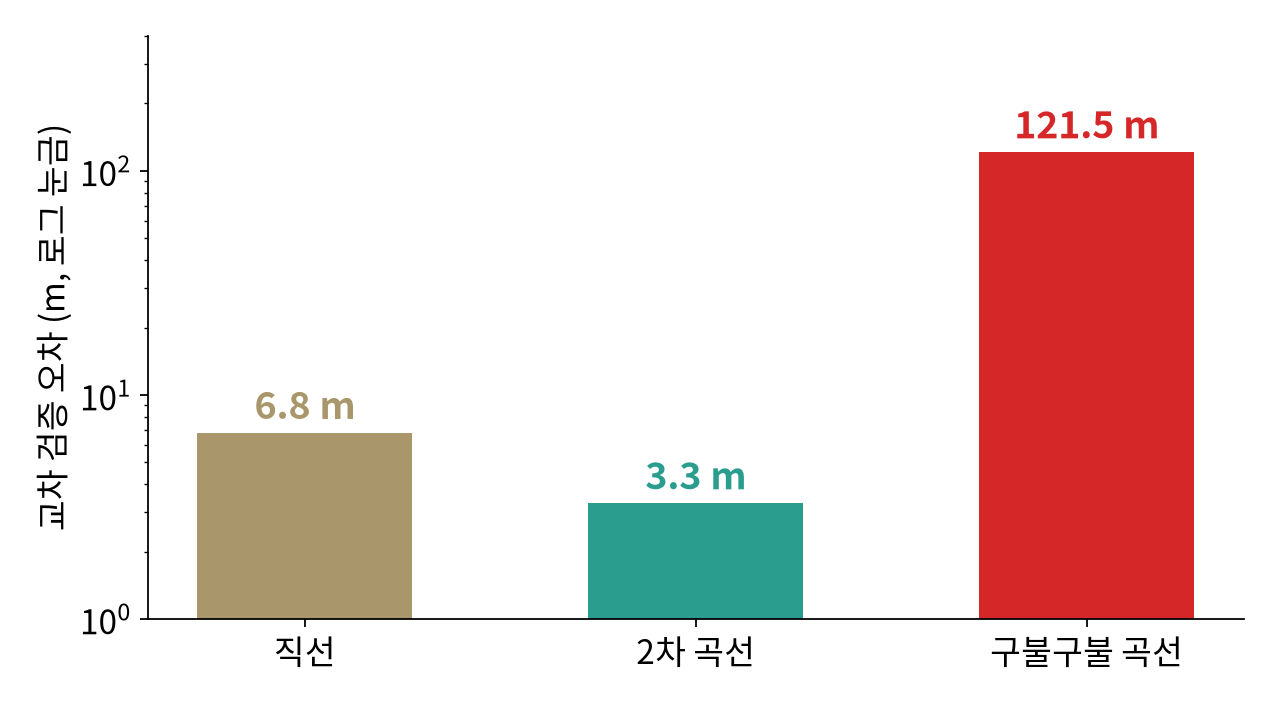
\includegraphics[width=0.56\linewidth]{of_cv.png}\par\vskip0.3em
{\large 직선 6.8 m \quad 2차 곡선 \kb{3.3 m} \quad 구불구불 곡선 \kq{121.5 m} \qquad $\to$ \kb{2차 곡선}}
\vfill
\note{세 모델의 교차 검증 오차입니다. 직선은 6.8미터, 2차 곡선은 3.3미터, 구불구불 곡선은 121.5미터입니다. 구불구불 곡선은 점 8개로 학습하면 숨긴 점 근처에서 크게 출렁여서 오차가 폭발합니다. 세로축이 로그 눈금이라는 점에 주의하세요. 가장 작은 2차 곡선을 고릅니다. 새 데이터를 하나도 쓰지 않고, 새 데이터에서 1등이었던 모델을 골라냈습니다 \pref{table}.}
\end{frame}

% --- 차수 전부
\begin{frame}{차수를 1부터 9까지 전부 재 보면}
\vfill
\centering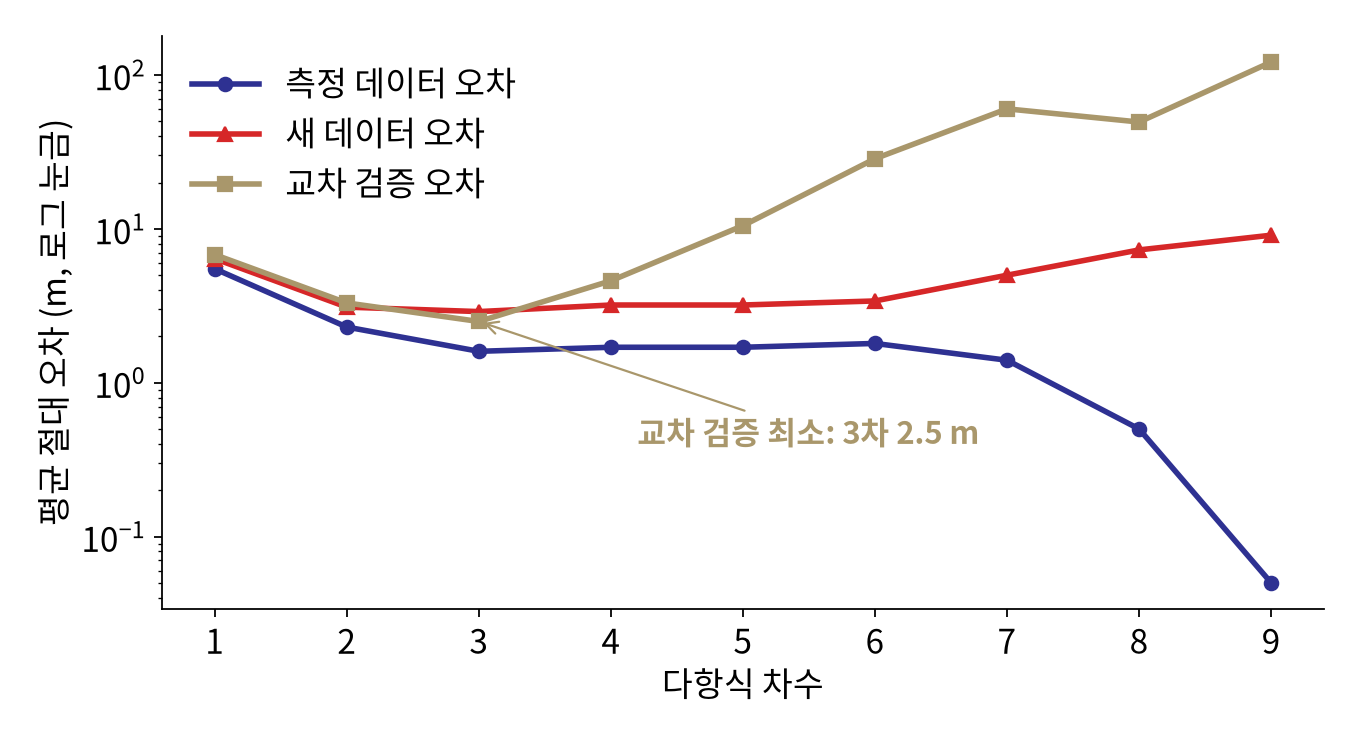
\includegraphics[width=0.6\linewidth]{of_sweep.png}\par\vskip0.3em
{\large 측정 오차는 계속 줄지만, 교차 검증 오차는 \kb{U자}: 2차 3.3 m · 3차 2.5 m 에서 바닥}\\[0.2em]
{\small 둘이 비슷하면 단순한 쪽을 고른다 \quad (9차의 측정 오차 0 m 는 로그 눈금이라 바닥에 붙여 그렸다)}
\vfill
\note{1차부터 9차까지 전부 재 봤습니다. 파란 측정 데이터 오차는 차수를 올릴수록 계속 줄어서 9차에서 0이 됩니다. 반면 노란 교차 검증 오차는 U자 모양입니다. 3차가 2.5미터로 가장 작고 2차가 3.3미터로 거의 같습니다. 점이 10개뿐이라 이 정도 차이는 잡음 수준이고, 둘이 비슷하면 더 단순한 2차를 고르는 게 보통입니다. 실제로 물리 법칙도 2차입니다. 빨간 새 데이터 오차도 같은 U자를 그립니다. 교차 검증이 새 데이터 오차를 잘 흉내 낸다는 뜻입니다.}
\end{frame}

\section{연습}
% --- 문제풀이
\begin{frame}{문제풀이}
\vfill
\begin{enumerate}
\item 점 4개 $(1,2), (2,3), (3,5), (4,6)$ 에 모델 $h = 1.4x + 0.5$. \; (a) 네 오차 $|h - y|$ 는? \; (b) MAE 는?\vskip0.8em
\item 어떤 모델의 측정 데이터 오차 1 m, 교차 검증 오차 40 m. 다른 모델은 12 m, 13 m. 각각 무엇인가?\vskip0.8em
\item 점 20개로 5겹 교차 검증을 한다. 한 번 학습할 때 몇 개로 학습하고 몇 개로 검증하나? 모델은 모두 몇 번 학습하나?\vskip0.8em
\item 점 10개에 9차 다항식이 항상 모든 점을 지날 수 있는 이유는?
\end{enumerate}
\vfill
\note{1번 답. 예측은 1.9, 3.3, 4.7, 6.1이라 오차는 0.1, 0.3, 0.3, 0.1이고 MAE는 0.8을 4로 나눈 0.2입니다. 2번 답. 첫 번째는 측정 오차는 작은데 교차 검증 오차만 크니 과대적합, 두 번째는 둘 다 크니 과소적합입니다. 3번 답. 20개를 4개씩 5조각으로 나누니 16개로 학습하고 4개로 검증합니다. 모델은 다섯 번 학습합니다. 4번 답. 9차 다항식에는 고를 수 있는 숫자가 w0부터 w9까지 10개라서, 점 10개의 방정식 10개를 모두 만족시킬 수 있습니다.}
\end{frame}

% --- 실습
\begin{frame}{실습}
\vfill
\centering\begin{tabular}{rl}
\large 1 & 슬라이드 데이터: 직선 · 2차 · 9차를 맞추고 MAE 재기 $\to$ 성적표 재현 \pref{table}\\[0.5em]
\large 2 & 5겹 교차 검증 직접 구현 $\to$ 6.8 / 3.3 / 121.5 m 재현\\[0.5em]
\large 3 & 실제 자동차 50대의 속도와 제동거리: 교차 검증으로 차수 고르기
\end{tabular}\vskip1em
cars (Ezekiel, 1930; R 기본 데이터) \\[0.4em]\href{https://colab.research.google.com/github/SuminHan/book-ml/blob/main/slides/v2/ml1/week02/overfitting/lab/overfitting.ipynb}{\textcolor{ksagolddk}{▶ Colab에서 실습 노트북 열기}}
\vfill
\note{실습은 세 부분입니다. 첫째, 오늘의 제동거리 데이터에 직선, 2차, 9차를 맞추고 MAE를 직접 계산해서 성적표를 재현합니다. 둘째, 5겹 교차 검증을 반복문으로 직접 구현해서 6.8, 3.3, 121.5미터를 재현합니다. 셋째, 1920년대에 실제로 잰 자동차 50대의 속도와 제동거리 데이터로, 교차 검증을 써서 알맞은 차수를 고릅니다.}
\end{frame}

\section{정리}
% --- 정리
\begin{frame}{정리}
\vfill
\centering\large\begin{tabular}{l}
\kb{과소적합} \quad 너무 단순해서 가진 데이터도 못 따라간다 (두 오차 모두 큼)\\[0.5em]
\kq{과대적합} \quad 가진 데이터를 외워서 새 데이터를 틀린다 (측정 오차만 작음)\\[0.5em]
학습에 쓴 데이터의 오차로는 모델을 고를 수 없다\\[0.5em]
\textbf{교차 검증} \quad 돌아가며 숨겨 두고 맞혀 본 오차의 평균으로 고른다
\end{tabular}
\vfill
\note{정리합니다. 과소적합은 모델이 너무 단순해서 가진 데이터도 못 따라가는 것, 과대적합은 가진 데이터를 외워서 새 데이터를 틀리는 것입니다. 학습에 쓴 데이터의 오차는 외울수록 작아지니까 모델을 고르는 기준이 될 수 없습니다. 그래서 데이터를 돌아가며 숨겨 두고 맞혀 보는 교차 검증으로 고릅니다. 5주차에 정규화와 함께 교차 검증을 다시 자세히 다룹니다.}
\end{frame}
\end{document}
